\chapter{Background \& Related Work}

In this chapter, we first provide a brief introduction to harmony and chords in music and the importance of recognising them. We then discuss the different ways in which music can be represented as input to a machine learning model. We then provide an overview of the field of automatic chord recognition (ACR). We discuss the datasets, models, and evaluation metrics that are commonly used in ACR and the challenges that are faced in this field. Finally, we discuss related work in the generation of synthetic data for music transcription tasks.

\section{Background}

\subsection{Harmony, Chords and Chord Recognition}

Harmony is the combination of simultaneously sounded notes. A common interpretation of such sounds is as a chord, especially in Western music. Chords can be thought of as a collection of at least two notes, built from a root note often with the third and fifth degrees of the scale. They can be extended with any notes but the most common are the seventh, ninth, eleventh and thirteenth upper extensions. A chord's \emph{quality} is determined by the intervals between notes in the chord irrespective of the root note. The most common chord qualities are major and minor, based off of the major and minor scales but many others exist such as diminished, augmented, and suspended chords. Chords can be played in inversion, where the root note is not the lowest note, and can be played in many voicings, where the notes are played in different octaves. In this work, we represent chords using Harte notation~\citep{HarteNotation} as described in Section~\ref{sec:chord-annotations}.

Chords are an important part of music. They provide a harmonic context for a melody, and can be used to convey emotion, tension and release. They are also important for improvisation where musicians will often play notes that fit the chord progression such that they a create pleasing sound. Many forms of musical musical notation rely on chords. Contemporary guitar music, or any accompaniment, can often be represented by just a chord sequence. Lead sheets are a form of notation which strip down a piece of music to its chord sequence and the melody. Lead sheets are often used for improvisation, especially in jazz music and chords are integral to this notation. A lead sheet for `Yesterday' by The Beatles can be found in Figure~\ref{fig:lead_sheet_example}. Chords are also important for songwriting, where a chord progression can be the basis of a song. They also play an important role in music analysis, where the harmonic structure of a piece can be analysed to better understand the composer's intentions, and to understand why we enjoy certain kinds of music.

Chord recognition is the task of identifying the chords present in a piece of music. This can be useful for creating notated versions of songs, for music analysis, for music recommendation and for music generation. Those wishing to learn pieces of music may start by visiting websites such as Ultimate Guitar\footnote{\url{https://www.ultimate-guitar.com/}} where users submit chord annotations for songs. Music researchers may wish to analyse the harmonic structure of a piece of music, or analyse the changes in common chord sequences over time. Music recommendation systems may recommend songs based on their harmonic content as similar music will often have similar harmonic content. For example, modern pop music famously uses many similar chords~\footnote{\url{https://www.youtube.com/watch?v=oOlDewpCfZQ}} while jazz music is known for its complex and rich exploration of harmony. Music generation systems can generate audio based on a given harmonic structure~\citep{MusicGenChord}.

All of the above motivate the need for accurate chord recognition systems. Annotations from online sources can be of varying quality and may not be available for all songs. The task of annotating chords is time-consuming and requires a trained musician. Automatic chord recognition systems have the potential to alleviate these problems by providing a fast, accurate and scalable solution.

\begin{figure}[H]
    \centering
    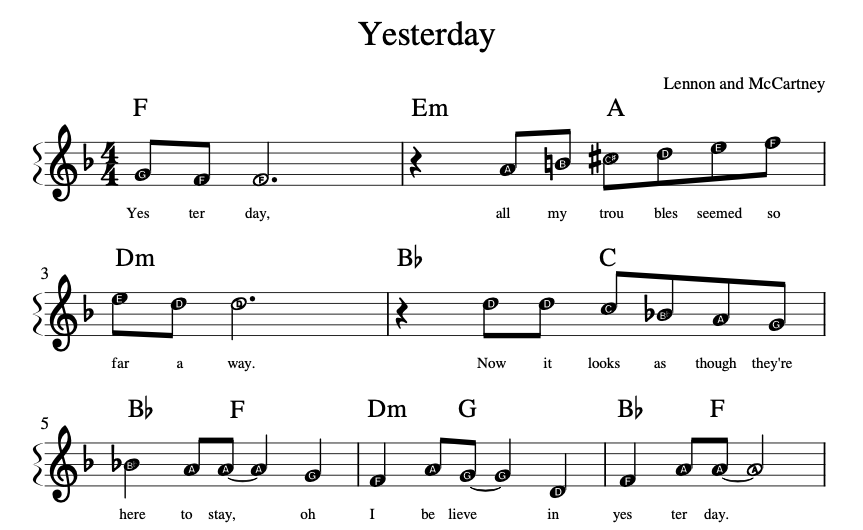
\includegraphics[width=0.8\textwidth]{figures/lead_sheet_example.png}
    \caption{An example of a lead sheet for `Yesterday' by the Beatles. We can see chords written above the stave and the melody written in standard musical notation. Such a chordal representation is useful for musicians who want to learn and perform songs quickly or improvise around them.}\label{fig:lead_sheet_example}
\end{figure}

% Lead sheets are most notably used in jazz music where their origins lie. They date back to the mid 20th century, and were originally called `fake sheets' because they were used by musicians to `fake' their way through a song~\citep{RealBookPodcast}. Any jazz musician worth their salt owns a `real book', so called to distinguish it from the fake books that were used in the past. Real books contain lead sheets for hundreds of jazz standards, and are still an essential tool for any seasoned jazz musician. 

% More recently they have served as a useful tool for musicians in other genres too, such as pop and rock, who want to learn and perform songs quickly and easily. They allow efficient communication of the important elements of a song, without the need for a full score, encouraging further improvisation and personalisation of the song.

% Lead sheets do not contain all the information of a full score, such as dynamics, articulation, or specific voicings of chords. Furthermore, they are not suitable for all types of music, such as classical music, where a full score is necessary to convey the composer's intentions, or rap music where the lyrics and beat are normally the most important elements. However, they are a useful tool for many musicians, and are a common way of representing music for both learning and performing.

% \subsection{Automatic Music Transcription}

% Automatic Music Transcription (AMT) is a field within Music Information Retrieval (MIR) that aims to construct models that convert musical audio into symbolic representations.~\citep{ComprehensiveReviewMusicTranscription} provide a comprehensive review of different forms of transcription. For lead sheet transcription, we are interested in their highest level of transcription: notation-level. We want to be able to take an audio recording of a song and generate a lead sheet that contains the melody and harmony of the song. This is a challenging task, as it requires the model to isolate and transcribe a melody, transcribe the chordal information, and then combine these two elements into a coherent lead sheet where the melody and harmony are aligned in time/beat.

% There are three sub-fields of musical transcription that are of interest to lead sheet generation: Automatic Chord Recognition (ACR), Melody Transcription (previously called F0 estimation) and Beat Detection.


\subsection{Music Features}\label{sec:background-features}

Recorded music can be represented in a variety of ways as input to a machine learning model. The simplest is to leave the data as a waveform - a time-series of amplitudes. Data in the raw audio domain has been successfully applied in generative models such as Jukebox~\citep{Jukebox} and RAVE~\citep{RAVE}.

\textbf{Spectrogram}: A common representation of audio data is the spectrogram. A spectrogram is a conversion of the time-series data into the time-frequency domain, calculated via a short-time Fourier transform (SFTF). Spectrograms are commonly used in many audio processing tasks, such as speech recognition, music recognition~\citep{ShazamSpectrogram} and music transcription, specifically polyphonic transcription~\citep{PianoTranscriptionWithTransformer}. However, as noted by~\citet{20YearsofACR}, only logarithmic spectrograms have been used in ACR tasks.

\textbf{CQT}: A common version of the spectrogram used in music transcription is the Constant-Q Transform (CQT), originally proposed by~\citet{CQT}. The CQT is a version of a spectrogram with frequency bins that are logarithmically spaced and bin widths that are proportional to the frequency. This is motivated by the logarithmic nature of how humans perceive pitch: a sine wave has double the frequency is perceived as one octave higher. The CQT is used in many music transcription tasks, such as automatic chord recognition~\citep{FirstDeepLearningCQT}, and a popular alternative, Melspectrograms, have found use in melody transcription~\citep{PianoTranscriptionWithTransformer}. An example CQT from the dataset used in this work is shown in Figure~\ref{fig:cqt_example}.

\begin{figure}[H]
    \centering
    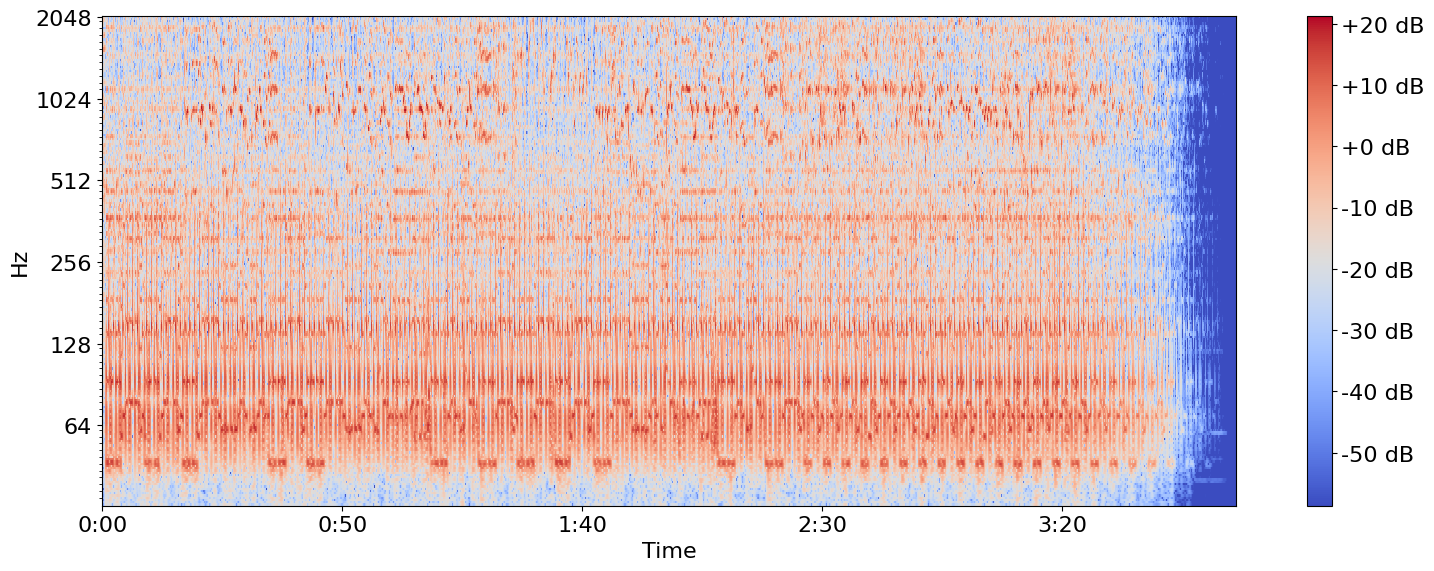
\includegraphics[width=1\textwidth]{figures/sample_cqt.png}
    \caption{A sample CQT of `Girls Just Wanna Have Fun' by Cyndi Lauper from the dataset used in this work. We can see the log-spaced frequency bins on the y-axis. There is clear structure and repetition in the song, particularly in the lower frequencies, which can be attributed to a regular drum groove and bass instruments. This is typical of songs in this dataset. Such structure and repetition gives an idea of the patterns a machine learning model may look for to identify chords.}~\label{fig:cqt_example}
\end{figure}

\textbf{Chroma Vectors}: Chroma vectors are a 12-dimensional time-series representation, where each dimension corresponds to a pitch class. Each element represents the strength of each pitch class in the Western chromatic scale in a given time frame. Such features have been generated by deep learning methods~\citep{BalanceRandomForestACR} or by hand-crafted methods~\citep{NNLSChroma} and have seen use in recent ACR models~\citep{HarmonyTransformer}.

\textbf{Generative Features}: More recently, features extracted from generative models have been used as input~\citep{MelodyTranscriptionViaGenerativePreTraining}. The proposed benefit is that the vast quantities of data used to train these models allows for rich representations of the music. This work uses features from JukeBox~\citep{Jukebox} to train a transformer~\citep{AttentionIsAllYouNeed} for both melody transcription and chord recognition. They then combine these into a lead sheet generation model. They found that these features outperformed hand-crafted features in melody transcription tasks but did not perform experiments in ACR.

\section{Related Work}

\subsection{Automatic Chord Recognition}\label{sec:background-acr}

Chord recognition is a difficult task. Which chord is playing when is inherently ambiguous. Different chords can share the same notes and the same chord can be played in different ways. The same chord can also be played in different contexts, such as a different key, time signature or on a different instrument. Whether a melody note is part of a chord is ambiguous and whether a melody alone is enough to imply harmonic content is also ambiguous. In order to identify a chord, information across time must be considered as the chordal information may be spread over time. For example, a chord may vamped or arpeggiated. Audio contains many unhelpful elements for chord recognition such as reverb, distortion and percussion. Combined with the lack of labelled data, this makes chord recognition a challenging task.

\citet{20YearsofACR} provide an overview of ACR since the seminal work of~\citet{FujishimaACR} in 1999 up to 2019, and provide suggestions for future avenues of research.

% Among them are the lack of exploration of feature and chord representations and the imbalance with chords classes present in chord datasets.

\textbf{Datasets}: Sources of data that have seen common use in ACR relevant to this work include:
\begin{itemize}
    \item \emph{Mcgill Billboard}: over 1000 chord annotations of songs randomly selected from the Billboard `Hot 100' Chart between 1958 and 1991.~\citep{McgillBillboard}
    \item \emph{Isophonics}: 300 annotations of songs from albums by The Beatles, Carole King and Zweieck.~\citep{Isophonics}
    \item \emph{RWC-Pop}: 100 pop songs with annotations available\footnote{\url{https://github.com/tmc323/Chord-Annotations}} for chords.~\citep{RWC}
    \item \emph{USPop}: 195 annotations of songs chosen for popularity.~\citep{USPop}
    \item \emph{JAAH}: 113 annotations of a collection of jazz recordings.~\citep{JAAH}
    \item \emph{HookTheory}: 50 hours of labelled audio in the form of short musical segments, crowdsourced from an online forum called HookTheory\footnote{https://www.hooktheory.com/}.~\citep{MelodyTranscriptionViaGenerativePreTraining}
\end{itemize}

Other small datasets also exist. Many of these have been compiled together into the \emph{Chord Corpus} by \citet{Choco}, with standardised annotation formats.

A problem frequently encountered in ACR is the lack of labelled data. This is due to the difficulty and time associated with labelling data aligned in time and the legal sensitivity of the data involved. Data has been scaled up using augmentation and semi-supervised learning~\citep{ScalingUpSemiSupervisedLearning} with some success. Research has been done into the use of synthetic data~\citep{MusicGenTrainingData,AnnotationFreeSyntheticData} and supervised learning~\citep{MERTSupervisedLearning} for MIR tasks, but not for ACR. 

Another problem is that the existing data is often imbalanced, with a large number of common chords like major and minor chords and fewer chords like diminished and augmented chords, or chords with upper extensions and inversions. This can lead to models that are biased towards predicting major and minor chords. Attempts to address such a long-tailed distribution have been made by re-weighting classes~\citep{ACRLargeVocab1}, adding a term in the loss function rewarding the identification of individual notes~\citep{StructuredTraining,ACRLargeVocab1}, re-sampling training examples to balance chord classes~\citep{BalanceRandomForestACR} and curriculum learning~\citep{CurriculumLearning}.

\textbf{Models}: A variety of machine learning methods have been applied to such datasets. Older methods often use hidden Markov models (HMMs)~\citep{ACRHMM} but more recent methods use deep learning. Convolutional neural networks (CNNs) and recurrent neural networks (RNNs) are used together in many works~\citep{ACRCNNRNN1,ACRLargeVocab1,StructuredTraining} with a CNN performing feature extraction from a spectrogram feature and an RNN sharing information across frames. More recently, transformers have been applied to the entire process~\citet{MelodyTranscriptionViaGenerativePreTraining, HarmonyTransformer, AttendToChords}.

\textbf{Decoding}: HMMs still see use as a decoder operating on the frame-wise probability distributions over chords generated by the model~\citep{BalanceRandomForestACR}. Other works have used conditional random fields (CRF) in their place to model the dependencies between chords~\citep{ACRLargeVocab1}.

\textbf{Evaluation}: Evaluation is typically done using recall of correct chord predictions, with recalls weighted by the commonality of each class. More music-aware measures provide further insights such as the recall of the correct root note, third, seventh or mirex, a metric which checks whether a predicted chord has at least 3 notes in common with the label chord. These are all implemented by~\citet{mir_eval} in the \texttt{mir\_eval} library~\footnote{\url{https://mir-evaluation.github.io/mir_eval/}}. Qualitative evaluation is also often carried out.

% \subsection{Lead Sheet Transcription}

% Older work has attempted to automatically produce lead sheets~\citep{LeadSheet2008,LeadSheet2009}. They use hand-crafted feature extractions and probabilistic models for melody and chord classification. AMT has developed dramatically since this work which leaves much room for improvement.

% \citep{MelodyTranscriptionViaGenerativePreTraining} is the only recent work we found that produces a full lead sheet generation model. They propose the use of features extracted from middle layers if Jukebox~\citep{Jukebox} which were found to lead to the best performance in downstream tasks~\citep{JukeBoxFeatureExtraction}. These features are used to train a transformer, with a primary focus on melody transcription. The model and code is available\footnote{\url{https://github.com/chrisdonahue/sheetsage/tree/main}}. They use the same methodology to train an ACR model, and combine these with beat detection and engraving software to produce a lead sheet.

% The authors found the use of these generative pre-trained features to be beneficial for melody transcription. However, they use community-submitted annotations from an online forum, presumably for lack of a better alternative, whose quality and variety may be lacking. The nature of this data means that the model is only trained on 24 second audio clips, which limits performance on longer segments of audio. The authors claim that the overall model performs well, especially in the verses and choruses of pop music where vocal lines are loud and clear, and that performance across genres is surprisingly good given the pop-centric dataset. However, further analysis is omitted and if the dataset contains music with few songs with more complex harmonic structures such as jazz music, then the model will produce overly simplistic representations of the chords. Crucially, the work does not explore ACR models beyond simply copying their method and dataset used in melody transcription and there is no quantitative evaluation of performance in ACR. Furthermore, the system can struggle with melody lines shifting between instruments, quiet vocal lines.

\subsection{Synthetic Data Generation}